\documentclass[12pt,a4paper]{report}
\usepackage{graphicx}
\usepackage{tikz}
\usetikzlibrary{matrix}
\begin{document}
\begin{titlepage}
	\centering
	\includegraphics[width=0.15\textwidth]{example-image-1x1}\par\vspace{1cm}
	{\scshape\LARGE Carnegie University \par}
	\vspace{1cm}
	{\scshape\Large Reinforcement Learning Project\par}
	\vspace{1.5cm}
	{\huge\bfseries Frozen Lake\par}
	\vspace{2cm}
	{\Large\itshape Hao Xu\par}
	\vfill
	Course-based project in\par
	10703 Reinforcement Learning\textsc{Brown}

	\vfill

% Bottom of the page
	{\large \today\par}
\end{titlepage}


{\bfseries\Large Background}
\vspace{0.5cm}

The FrozenLake environment is from the OpenAI Gym Environment API. For more information on the Gym and the API see: https://gym.openai.com/. 

There are three different tile types: frozen, hole, and goal. When the agent lands on a frozen tile it receives 0 reward. When the agent lands on a hole tile it receives 0 reward and the episode ends. When the agent lands on the goal tile it receives +1 reward and the episode ends. 

Map size: $4\times4$ and $ 8\times8$

States are represented as integers numbered from left to right, top to bottom starting at zero. So the upper left corner of the 4x4 map is state 0, and the bottom right corner of the 4x4 map is state 15.


\vspace{0.5cm}
{\bfseries\Large SARSA method}
\vspace{0.5cm}

I'm using Policy Iterative Method to practice the environment, for more information of the method, please review the book at page 87:

http://webdocs.cs.ualberta.ca/~sutton/book/bookdraft2016sep.pdf

Figure 1 shows the main algorithms used in the practice.

\includegraphics[scale=0.5]{algorithm}
\vspace{0.1cm}

\includegraphics[scale=0.5]{algorithm2}

In the deterministic versions, the up action will always move the agent up, the left will always move left, etc. In the stochastic versions, the up action will move up with probability 1/3, left with probability 1/3 and right with probability 1/3.

The left side of figure 2 shows the value function color plot for 4x4 determinstic, and 4x4 stochastic version environment. And The right side is their optimal policy respectively.

\includegraphics[scale=0.4]
{Deterministic-4x4}
\includegraphics[scale=0.4]{stachostic-4x4}

\begin{figure}[!htb]
	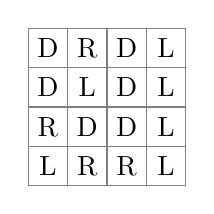
\begin{tikzpicture}
	\draw[step=0.5cm,color=gray] (-1,-1) grid (1,1);
	\node at (-0.75,+0.75) {D};
	\node at (-0.25,+0.75) {R};
	\node at (+0.25,+0.75) {D};
	\node at (+0.75,+0.75) {L};
	\node at (-0.75,+0.25) {D};
	\node at (-0.25,+0.25) {L};
	\node at (+0.25,+0.25) {D};
	\node at (+0.75,+0.25) {L};
	\node at (-0.75,-0.25) {R};
	\node at (-0.25,-0.25) {D};
	\node at (+0.25,-0.25) {D};
	\node at (+0.75,-0.25) {L};
	\node at (-0.75,-0.75) {L};
	\node at (-0.25,-0.75) {R};
	\node at (+0.25,-0.75) {R};
	\node at (+0.75,-0.75) {L};

	\end{tikzpicture}
\end{figure}

\begin{figure}[!htb]
	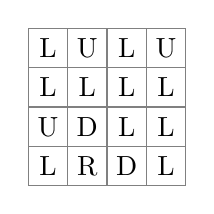
\begin{tikzpicture}
	\draw[step=0.5cm,color=gray] (-1,-1) grid (1,1);
	\node at (-0.75,+0.75) {L};
	\node at (-0.25,+0.75) {U};
	\node at (+0.25,+0.75) {L};
	\node at (+0.75,+0.75) {U};
	\node at (-0.75,+0.25) {L};
	\node at (-0.25,+0.25) {L};
	\node at (+0.25,+0.25) {L};
	\node at (+0.75,+0.25) {L};
	\node at (-0.75,-0.25) {U};
	\node at (-0.25,-0.25) {D};
	\node at (+0.25,-0.25) {L};
	\node at (+0.75,-0.25) {L};
	\node at (-0.75,-0.75) {L};
	\node at (-0.25,-0.75) {R};
	\node at (+0.25,-0.75) {D};
	\node at (+0.75,-0.75) {L};

	\end{tikzpicture}
\end{figure}

The policy iteration method is going to take 85 value steps and 6 improve steps, while the value iteration method is only taking 22 steps.




\end{document}
